\documentclass[11pt,a4paper]{article}
\usepackage[margin=25mm]{geometry}
\usepackage{amsmath,amssymb}
\usepackage{booktabs}
\usepackage{siunitx}
\usepackage{microtype}
\usepackage{tikz}
\usepackage{pgfplots}
\pgfplotsset{compat=1.16}
\usetikzlibrary{arrows.meta,positioning,calc,fit,backgrounds}
\usepackage[colorlinks,linkcolor=blue!45!black]{hyperref}

\definecolor{done}{RGB}{20,140,110}
\definecolor{todo}{RGB}{200,90,20}
\definecolor{cam}{RGB}{20,110,180}
\definecolor{soft}{RGB}{130,145,155}

\title{\bfseries Cloud coverage from stellar intensity time series\\[2mm]
\large Status of the GAIA implementation, and what remains}
\author{Memo --- GAIA Data Center}
\date{15 September 2026 \\ \small(fifth revision; first issued 10 September 2026)}

\begin{document}
\maketitle

\begin{abstract}
\noindent
Cloud attenuates starlight, so the brightness of a known star measures the
optical depth along that line of sight. This memo records what is implemented
and verified in GAIA, what is stored, and what remains. The estimation chain is
complete and pinned against the AIDA reference implementations to
\SI{1e-6}{\degree} in the ephemeris and \SI{1e-6}{px} in the projection, for all
six lens models in live use. Since the first issue the photometric model has
been strengthened where it was weakest: the sky under a star is now a bilinear
plane rather than a constant, every measurement carries the scatter of its own
fit residuals so a star can be tested against the frame's own noise instead of
being trusted blindly, and the solar and lunar state at the station is computed
and stored per frame. Storage, both diagnostic plots, and the writer that
fills them all exist, and the writer has been running in production since
10 September: \num{2.4} million measurements over \num{71} cameras, every one
of them detecting stars. The clear-sky reference exists too, and after three
faults were found and fixed it is accumulating: 63 fits over 21 cameras at the
time of writing, at \num{0.166} magnitudes per air mass in each colour channel
and \num{0.186} in the mean against a literature
clear sky near \num{0.20}, a figure the estimator was never told. Every measurement a fitted
camera-night explains now carries a vertical optical depth --- \num{33287} of
\num{2.47} million, rising as the backfill sweeps older nights --- with
saturated, undetectable and unexplained measurements deliberately left null
rather than guessed, and the depth capped at 6 where the sky is already opaque.
Those depths can now be read one at a time as well as in aggregate, which for
most of this revision's life they could not: see Sec.~\ref{sec:audit}. What
remains is to spend that number: no cloud weight yet reaches the
composite and no cloud map is published. Neither is research.
\end{abstract}

\section{What changed since the first issue}

Four things in the estimation and storage layers, added between the first and
second issues:

\begin{enumerate}
  \item \textbf{Bilinear background.} The fit went from 7 to 10 parameters. The
    sky under a star is now $b_0+b_xX+b_yY+b_{xy}XY$ about the patch centre,
    which was the cheap improvement flagged as an open issue in the first issue
    and is now closed.
  \item \textbf{Detectability.} Each fit reports the standard deviation of its
    own residuals and two signal-to-noise ratios built from it, so a peak that
    is merely noise can be refused rather than fed to the cloud estimate as a
    clear sky.
  \item \textbf{Lunar and solar state per frame.} A lunar ephemeris and a
    \texttt{frame\_sky} table record where the Moon and Sun were, how bright the
    Moon was, and a geometric moonlight proxy, for every measured frame.
  \item \textbf{The composite weight chain gained a manual per-camera quality
    factor}, a power of two from 1 to $1/256$ set by the operator. It is
    unrelated to cloud, but it settles the question of how an extra per-camera
    factor enters the sum, and the cloud weight will enter the same way.
  \item \textbf{The writer exists} (Sec.~\ref{sec:writer}). The tables are no
    longer empty, which moves the blocking item from ``nothing measures'' to
    ``nothing yet turns a measurement into an optical depth''.
\end{enumerate}

\noindent Since the second revision, three days later, the writer has been
deployed and has produced enough data to answer questions the memo could only
pose:

\begin{enumerate}
  \item \textbf{The pointing conclusion needed narrowing.} The second revision
    generalised from the only two cameras then measured, and both happened to
    belong to the one station family in the archive with a drift problem. Across
    66 cameras, 47 point true to better than half a pixel
    (Table~\ref{tab:pointing}).
  \item \textbf{The air-mass confound is measured} rather than predicted, and
    its spread across stars is itself the argument for which remedy to build
    (Sec.~\ref{sec:airmass}).
  \item \textbf{The composite moved into the browser}, so a cloud weight now has
    two places to be applied rather than one, and unlike its neighbours it
    cannot be computed client-side (Sec.~\ref{sec:weightpath}).
\end{enumerate}

\noindent The fourth revision, a day later again, is mostly a correction. The
third reported the clear-sky reference as built and working. It was built; it
was not working. Three faults in the pass had left it stalled in production at
the twelve fits it had made in its first four hours, and the fault that hid this
was that the only evidence either way lived in two database tables nobody could
read without risking the service. All three are fixed and the reference is now
accumulating (Sec.~\ref{sec:stall}), and the evidence is now an API call.

\noindent The fifth revision carries two corrections of unequal weight. The
smaller: an uncapped depth had reached \num{40.25}, which is not a measurement
of cloud but of a star the reference expected and the frame never had. Depths
are now capped at 6 (Sec.~\ref{sec:depth}). The larger is about how any of
this gets checked at all. The series endpoint --- built, in the fourth
revision, precisely so the archive could be audited without opening the
database --- listed the optical depth as its twenty-second column and read it
from its twenty-seventh, which holds the solar elevation. Every depth it served
was the elevation of the Sun that evening: a smooth \num{-15} to \num{-18}
that reads as a perfectly plausible optical depth, which is exactly why it
survived review and two rounds of verification (Sec.~\ref{sec:audit}).

\section{The measurement chain}

Each stage below is a separate, testable step: a catalogue position becomes a
sky position, a sky position becomes a pixel through that camera's own lens
model, a pixel patch becomes a flux, and a series of fluxes becomes an optical
depth. All five are now built. What is not built is anything that reads the
last one.

\begin{figure}[h]
\centering
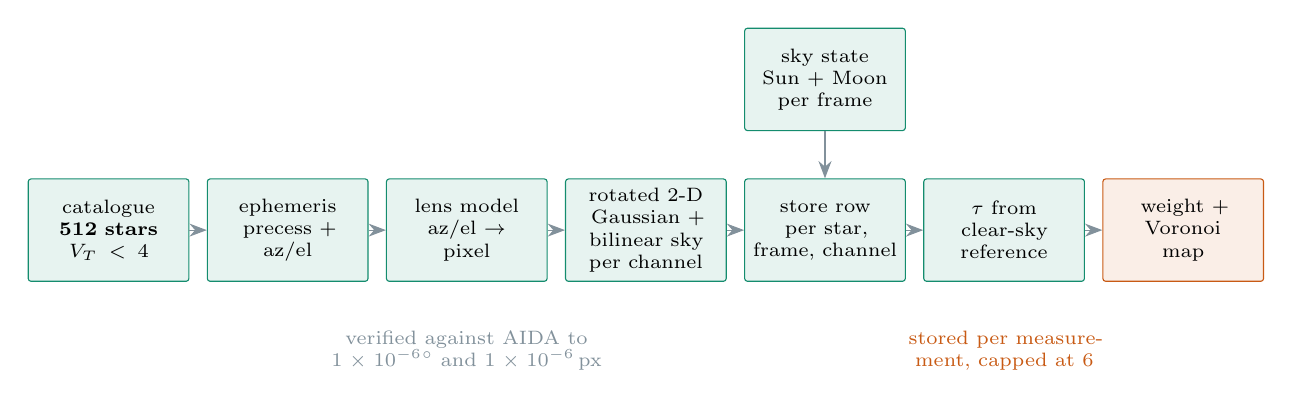
\begin{tikzpicture}[node distance=2.2mm,
  d/.style={draw=done,fill=done!10,rounded corners=1pt,align=center,font=\scriptsize,
            minimum height=13mm,text width=19mm,inner sep=2pt},
  t/.style={d,draw=todo,fill=todo!10},
  a/.style={-{Stealth[length=2.2mm]},soft}]
 \node[d] (cat) {catalogue\\ \textbf{512 stars}\\ $V_T<4$};
 \node[d,right=of cat] (eph) {ephemeris\\ precess +\\ az/el};
 \node[d,right=of eph] (proj) {lens model\\ az/el $\to$\\ pixel};
 \node[d,right=of proj] (fit) {rotated 2-D\\ Gaussian +\\ bilinear sky\\ per channel};
 \node[d,right=of fit] (store) {store row\\ per star,\\ frame, channel};
 \node[d,above=6mm of store] (sky) {sky state\\ Sun + Moon\\ per frame};
 \node[d,right=of store] (tau) {$\tau$ from\\ clear-sky\\ reference};
 \node[t,right=of tau] (out) {weight +\\ Voronoi\\ map};
 \draw[a] (cat)--(eph); \draw[a] (eph)--(proj); \draw[a] (proj)--(fit);
 \draw[a] (fit)--(store); \draw[a] (store)--(tau); \draw[a] (tau)--(out);
 \draw[a] (sky)--(store);
 \node[below=5mm of proj,font=\scriptsize,soft,text width=42mm,align=center]
   {verified against AIDA to \SI{1e-6}{\degree} and \SI{1e-6}{px}};
 \node[below=5mm of tau,font=\scriptsize,todo,text width=40mm,align=center]
   {stored per measurement, capped at 6};
\end{tikzpicture}
\caption{Green stages are implemented and tested; orange stages are not built.
The chain runs entirely from the camera's own calibration, so it needs no
additional instrumentation. The break has moved: a stored flux now becomes a
stored optical depth, and what remains unbuilt is everything downstream of that
number --- the composite weight and the published map.}
\label{fig:chain}
\end{figure}

\section{What is implemented and verified}

All of the following lives in \texttt{backend/starphot.rs} and is covered by the
Rust test suite (58 tests at the time of writing, 24 of them in this module).

\paragraph{Catalogue.} The AIDA \texttt{WISCAT1} payload is read directly:
\num{42072} stars, of which \textbf{512} are brighter than $V_T=4$, the
brightest at $V_T=-1.09$. Damaged or truncated payloads are refused rather than
misread.

\paragraph{Ephemeris.} Deliberate ports of the AIDA tool's
\texttt{precessJ2000ToDate} and \texttt{starAzZe}, so a star lands where the
calibration GUI puts it. Table~\ref{tab:verify} shows the agreement. An
independent physical check confirms Polaris tracks the observer latitude all day
to within the $\arcsin(\sin p/\cos\varphi)$ azimuth swing implied by its
\SI{0.74}{\degree} polar distance; a first attempt used a fixed
\SI{3}{\degree} bound and was wrong at \SI{78}{\degree}N.

\paragraph{Forward projection.} A port of \texttt{wisc\_lens.az\_el\_to\_pixel}.
The camera rotation is built as the explicit $R_y(\alpha)R_x(\beta)R_z(\gamma)$
product used by the reference; a hand-expanded version was wrong and the golden
tests caught it.

\paragraph{Photometry.} A rotated elliptical Gaussian on a bilinear sky, ten
parameters in all (Fig.~\ref{fig:gauss}), fitted by Levenberg--Marquardt with an
analytic Jacobian, started from intensity-weighted second moments. The angle
derivative is $\propto(\sigma_1/\sigma_2-\sigma_2/\sigma_1)$ and therefore
vanishes for a round star, so the damping is written to keep that case solvable
rather than singular. Results are returned in one canonical form, major axis
first with the angle wrapped to $[-90,90)$.

\paragraph{The sky under the star.} The background is now a plane with a
cross term, about the patch centre,
\begin{equation}
  B(X,Y) \;=\; b_0 + b_xX + b_yY + b_{xy}XY ,
\end{equation}
rather than a constant. Moonlight, twilight and an auroral arc all slope across
a patch, and a constant background forced to cover a gradient pushes the
difference into the amplitude, which is exactly the quantity being measured.
The tests plant gradients up to \num{2.4} counts per pixel and recover $b_x$ and
$b_y$ to \num{0.05} and the flux to \SI{2}{\percent}, with the amplitude
undisturbed. The reported \texttt{background} is the plane evaluated at the
fitted centroid, i.e.\ the sky actually under the star, while the four
coefficients are kept so the gradient itself can be examined later.

\paragraph{Detectability.} A fit always returns something; whether it is a star
is a separate question, and the answer has to come from the frame itself. Each
fit therefore reports $\sigma_r$, the standard deviation of its own residuals,
and two ratios against it,
\begin{equation}
  \mathrm{SNR}_A = \frac{A}{\sigma_r},
  \qquad
  \mathrm{SNR}_F = \frac{F}{\sigma_r\sqrt{4\pi\sigma_1\sigma_2}} ,
  \label{eq:snr}
\end{equation}
the denominator of the second being the noise integrated over the effective
area of the profile, which is the meaningful uncertainty on a photometric
point. \texttt{detectable(min\_snr)} requires both. This matters for cloud more
than for astrometry: under thick cloud a star does not vanish cleanly, it sinks
into the noise, and a fit to noise returns a small positive flux that
Eq.~\eqref{eq:tau} would read as \emph{thin} cloud. Refusing those samples is
the difference between an overcast sky reading as overcast and reading as
hazy.

Total intensity above background is the analytic integral
\begin{equation}
  F \;=\; 2\pi A\,\sigma_1\sigma_2 ,
\end{equation}
which is \emph{unchanged} by rotation because rotation preserves area. That is
the property an axis-aligned fit violates: forced to cover a tilted ellipse it
inflates both widths and overestimates the flux. Since $F$ is the measurement,
this matters directly.

\begin{table}[h]
\centering
\small
\begin{tabular}{llr}
\toprule
Quantity & Reference & Agreement \\
\midrule
Ephemeris, 4 stars $\times$ 3 epochs & \texttt{aidatools.js radecToAzZe} & \SI{1e-6}{\degree} \\
Precession of Sirius to date & \texttt{precessJ2000ToDate} & \SI{1e-9}{rad} \\
Forward projection, 6 lens models & \texttt{wisc\_lens.az\_el\_to\_pixel} & \SI{1e-6}{px} \\
Projection on \emph{real} data, 46 stars & Kiruna calibration model positions & \SI{0.0000}{px} median \\
Same, versus observed positions & the file's own residuals & \num{0.7411} vs \num{0.7411} px \\
Gaussian flux, noiseless & analytic $2\pi A\sigma_1\sigma_2$ & \SI{2}{\percent} \\
Gaussian flux, with noise & analytic & \SI{6}{\percent} \\
Position angle, $-70$ to $+80$\si{\degree} & planted truth & \SI{1}{\degree}, \SI{0.05}{px} \\
Background gradient, 4 cases & planted plane & \num{0.05} counts/px \\
Flux under a gradient & analytic & \SI{2}{\percent} \\
Residual scatter $\sigma_r$ & injected uniform noise & \SI{30}{\percent} \\
Lunar perigee, apogee over 400 d & \num{356400}--\SI{406700}{\kilo\meter} & bracketed \\
Lunar ecliptic latitude & orbital inclination \SI{5.3}{\degree} & $<\SI{5.6}{\degree}$ \\
Synodic month, Sun--Moon beat & \SI{29.53}{d} & \SI{0.4}{d} \\
One-based convention, 165 stars & file \texttt{model\_col\_px\_1based} & $-1.000000$, sd 0 \\
\bottomrule
\end{tabular}
\caption{Verification of the estimation chain. The fourth row is the strongest:
feeding a real calibration's own stored altitude/azimuth through the port
reproduces AIDA's own model pixel positions exactly, and the fifth reproduces
that file's published residuals, confirming the \texttt{col}$\leftrightarrow x$,
\texttt{row}$\leftrightarrow y$ and 1-based conventions that had to be inferred.}
\label{tab:verify}
\end{table}

\begin{figure}[h]
\centering
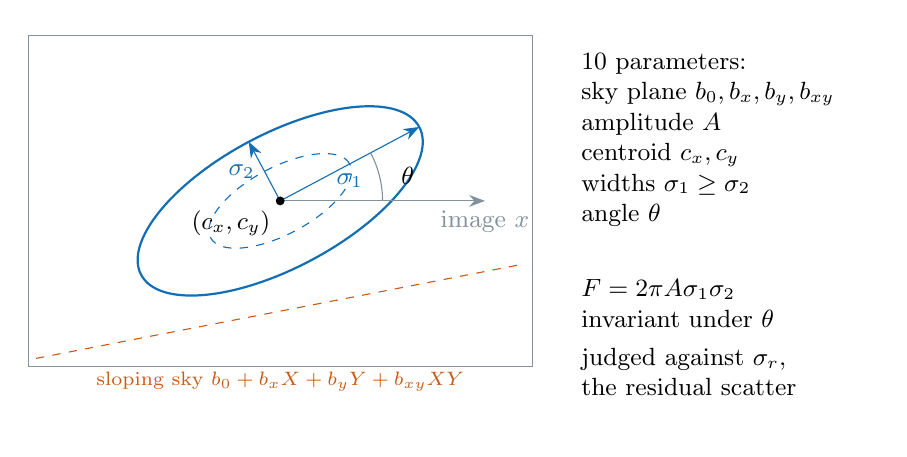
\begin{tikzpicture}[scale=1.0]
  \draw[soft] (-3.2,-2.1) rectangle (3.2,2.1);
  \begin{scope}[rotate=28]
    \draw[cam,thick] (0,0) ellipse (2.0 and 0.85);
    \draw[cam,dashed] (0,0) ellipse (1.0 and 0.425);
    \draw[cam,-{Stealth[length=2mm]}] (0,0) -- (2.0,0) node[midway,below,font=\small,cam] {$\sigma_1$};
    \draw[cam,-{Stealth[length=2mm]}] (0,0) -- (0,0.85) node[midway,left,font=\small,cam] {$\sigma_2$};
  \end{scope}
  \draw[soft,-{Stealth[length=2mm]}] (0,0) -- (2.6,0) node[below,font=\small,soft] {image $x$};
  \draw[soft] (1.3,0) arc (0:28:1.3);
  \node[font=\small] at (1.62,0.32) {$\theta$};
  \fill (0,0) circle (1.6pt) node[below left,font=\small] {$(c_x,c_y)$};
  \node[font=\small,align=left,anchor=north west] at (3.7,2.0)
    {10 parameters:\\ sky plane $b_0,b_x,b_y,b_{xy}$\\ amplitude $A$\\ centroid $c_x,c_y$\\ widths $\sigma_1\ge\sigma_2$\\ angle $\theta$};
  \node[font=\small,align=left,anchor=south west] at (3.7,-2.6)
    {$F=2\pi A\sigma_1\sigma_2$\\ invariant under $\theta$\\[1mm]
     judged against $\sigma_r$,\\ the residual scatter};
  \draw[todo,thin,dashed] (-3.1,-2.0) -- (3.1,-0.8);
  \node[font=\scriptsize,todo,anchor=north] at (0,-2.05) {sloping sky $b_0+b_xX+b_yY+b_{xy}XY$};
  \path (-3.2,-2.9) rectangle (7.6,2.2);
\end{tikzpicture}
\caption{The fitted star image. Rotation is needed because trailing during the
exposure, off-axis coma and astigmatism, and anisotropic binning all produce
elongated images. The reported angle is meaningless for a round star, which is
why \texttt{elongation()} is reported alongside it. The dashed line indicates
the sloping sky the star now sits on: a moonlit or auroral patch is not flat,
and a constant background would move that slope into $A$.}
\label{fig:gauss}
\end{figure}

\paragraph{Per-camera lens models.} The archive uses \textbf{six} different
models, and the field test must come from each camera's own calibration rather
than be assumed (Table~\ref{tab:models}). Brown--Conrady is rectilinear and
diverges outside its field: the archived \texttt{starvisor-bagdarin} calibration
returns \num{3.6e8} pixels at azimuth \SI{120}{\degree}, elevation
\SI{40}{\degree}, and \num{8.6e10} at azimuth \SI{250}{\degree}, elevation
\SI{20}{\degree}. Those are finite, and an early version returned them as star
positions. The forward-hemisphere test is deliberately \emph{not} applied to the
fisheye models, which legitimately image directions with $s_3\le0$: the archived
optmod-4 calibration has six such directions inside its frame.

\begin{table}[h]
\centering
\small
\begin{tabular}{lrrl}
\toprule
\texttt{optmod} & cameras & sky above \SI{5}{\degree} in field & note \\
\midrule
2  & 27 & \num{612}/\num{612} & all-sky fisheye \\
6  & 11 & \num{612}/\num{612} & all-sky fisheye \\
4  & 9  & \num{612}/\num{612} & 6 in-field directions with $s_3\le0$ \\
12 & 4  & \num{612}/\num{612} & all-sky fisheye \\
3  & 3  & \num{612}/\num{612} & all-sky fisheye \\
20 & 3  & \num{176}/\num{612} & rectilinear, diverges outside its field \\
\bottomrule
\end{tabular}
\caption{Lens models in live use, and measured sky coverage on a
\SI{10}{\degree} azimuth by \SI{5}{\degree} elevation grid.}
\label{tab:models}
\end{table}

\paragraph{The Moon.} A truncated Schlyter-style lunar series gives geocentric
right ascension, declination and distance, which the same ephemeris code turns
into azimuth and elevation at the station. From the elongation follow the phase
angle, the illuminated fraction, and an apparent magnitude by Allen's phase law
with the inverse-square distance term,
\begin{equation}
  m \;=\; -12.73 + 0.026\,|\alpha| + 4\times10^{-9}\,\alpha^4
          + 5\log_{10}\!\frac{d}{\SI{384400}{\kilo\meter}} ,
\end{equation}
$\alpha$ in degrees. A geometric proxy for how much moonlight reaches this
station's sky, the illuminated fraction times $\sin(\text{elevation})$ and zero
while the Moon is down, is stored alongside. No ephemeris library is available
here, so the series is checked against properties of the real orbit rather than
golden values: distance brackets perigee and apogee, ecliptic latitude stays
inside the orbital inclination, and the illuminated fraction beats against the
independently implemented solar longitude at \SI{29.53}{d}. That last test is
the strong one, because the synodic month only comes out right if both bodies
are right. It is worth saying plainly what this is for: moonlight raises the
background and its gradient, and a bright Moon low in the sky is one of the few
things that can imitate cloud in a stellar photometry series.

\section{What the AIDA calibrations do and do not provide}

The calibration HDF5 files contain \texttt{/selected\_stars}, whose columns are
named in the \texttt{selected\_\allowbreak star\_\allowbreak columns} root attribute: index, an
included-in-fit flag, altitude and azimuth, the measured star row and column,
J2000 right ascension and declination, magnitude, the model row and column, and
the three residuals. Names are in \texttt{selected\_\allowbreak star\_\allowbreak names}. This exists in
\textbf{27 of 59} archived calibrations, across 26 cameras; the remaining 32 are
UCalgary skymap-derived fits with no star data.

Crucially the \texttt{magnitude} column is the \emph{catalogue} $V$ magnitude,
not a measurement: Caph \num{2.27}, Schedar \num{2.23}, $\gamma$~Cas
\num{2.47}, exactly the published values, and no flux, ADU, instrumental
magnitude or background appears anywhere in the file. \textbf{There is therefore
no photometric zero point available}, which is why each star's clear-sky
reference must come from its own time series.

\section{What is stored}

The \texttt{star\_photometry} table holds one row per camera, frame, star and
colour channel, indexed so one star's series is a single index scan. It retains
the sky position (azimuth and elevation at the observation time, plus the J2000
position identifying the star), the image position twice over (predicted by the
lens model and found by the fit, with their separation), and every fitted
parameter including the background under the star, its three gradient
coefficients, both widths, the angle, the amplitude, the flux, the residual
scatter $\sigma_r$ and the two signal-to-noise ratios of
Eq.~\eqref{eq:snr}. A later re-measurement of the same star in the same frame
replaces the row rather than duplicating it.

A second table, \texttt{frame\_sky}, holds one row per camera and frame: the
solar elevation at the station and the full lunar state, azimuth, elevation,
illuminated fraction, phase angle, distance, apparent magnitude and the
moonlight proxy. It is keyed and indexed for the same kind of series scan, so a
brightness series can be read against the Moon that was up at the time without
recomputing any ephemeris.

Two choices are deliberate. \texttt{star\_key} is derived from the J2000
position, because the catalogue carries no identifier. And a star that is
\emph{looked for and not found} is still recorded, with a null fit and the
centroid distance kept: a star missing where the geometry says it should be
visible is itself evidence about the sky, and dropping the row would make an
overcast frame indistinguishable from an unmeasured one.

All four channels are measured, red, green, blue and the panchromatic mean,
because cloud extinction is wavelength dependent.

\section{The writer}
\label{sec:writer}

The pass lives in \texttt{backend/starpass.rs} and runs inside the archive
server. A frame is a candidate when its camera is enabled, located and
calibrated, when the frame lies inside the look-back window, and when it has no
row in \texttt{frame\_sky}. Every candidate is given its Sun and Moon row
immediately: that costs arithmetic only, it fills the sky record, and it is what
marks the frame as seen, so the pending set drains even for frames that will
never be worth photometering. Photometry itself runs only on the frames that
survive two further tests, a solar elevation at or below \SI{-6}{\degree} and a
minimum spacing from every frame of that camera already measured. The spacing is
checked against the database, not against a counter, so the sampling cadence
survives a restart.

The lens model is chosen by exactly the expression the projection and the
publisher use, an explicit operator selection when there is one and the
calibration covering the frame otherwise. A star is then measured through the
same optics the mosaic is drawn with. Reading the model shells out to
\texttt{h5dump}, so it is cached per calibration and carried between cycles.
Frames are decoded at full resolution; the \SI{256}{px} globe textures are
useless here, and nothing in this path may touch them.

\paragraph{Cost.} One cycle writes \num{400} sky rows and photometers six
\num{3840}$\times$\num{2160} frames in \SI{7}{\second}, about a second per frame
including the JPEG decode and the search over all \num{512} catalogue stars. At
the shipped settings, twelve frames every five minutes with a
\SI{250}{\milli\second} rest between them, the pass costs a few percent of one
core. It rests deliberately: the publisher takes sixteen cores under its own
lock, and a missed frame costs nothing when the quantity wanted is a time
series.

\paragraph{It is running.} The pass has been live on Revontuli since
10 September. As of 14 September at 06:30 UTC it holds

\begin{center}\small
\begin{tabular}{lr}
\toprule
sky rows (\texttt{frame\_sky}) & \num{132759} \\
photometry rows (\texttt{star\_photometry}) & \num{1622892} \\
frames photometered & \num{4761} \\
cameras & \num{71} \\
detections & \num{329121} \\
\bottomrule
\end{tabular}
\end{center}

\noindent Every one of the \num{71} cameras is producing detections and 53 of
them have passed a thousand. Kiruna is the richest at \num{416} rows per frame,
which is \num{104} stars in four colour channels. \SI{20.3}{\percent} of all
rows are detections, and \SI{20.2}{\percent} clear $\mathrm{SNR}_F>5$: almost
every fit that converges is comfortably above the noise, and almost every
failure is a patch with no star in it rather than a marginal one. That is the
behaviour the detectability design was aiming for.

The series are only now becoming long enough to work with. Counting per star per
camera, in the mean channel, there are \num{112} series with a hundred samples
or more, \num{167} with 50 to 99, and \num{877} with 20 to 49. A ninetieth
percentile is a real statistic from about twenty samples upward, so roughly
\num{1156} series can carry a clear-sky reference today, out of \num{8055} that
exist. The rest are short because the look-back window is \SI{48}{\hour} and the
cadence ten minutes; they lengthen on their own.

\begin{table}[h]
\centering
\small
\begin{tabular}{lr}
\toprule
mean pointing offset & cameras \\
\midrule
below \SI{0.5}{px} & 47 \\
\SI{0.5}{} to \SI{1}{px} & 16 \\
\SI{1}{} to \SI{1.5}{px} & 1 \\
above \SI{2}{px} & 2 \\
\bottomrule
\end{tabular}
\caption{Distance between the fitted centroid and the position the lens model
predicts, averaged per camera over confident detections, for the 66 cameras with
at least thirty of them. The projection is accurate to under half a pixel for
most of the archive.}
\label{tab:pointing}
\end{table}

\paragraph{Pointing: a few cameras have drifted, most have not.} The first two
cameras this pass ever measured, Bagdarin and Yurga, both showed a mean offset
of one to one and a half pixels that did not shrink with signal-to-noise, and
the second revision of this memo concluded from them that cameras drift after
calibration. With 66 cameras now measured instead of two, that conclusion needs
narrowing: it is true, but it is not the general case.
Table~\ref{tab:pointing} is the population. Forty-seven cameras point true to
better than half a pixel, and the per-frame shift is steady --- Kiruna sits at
$(+0.10,+0.03)$ px with a frame-to-frame scatter of \num{0.19} and \num{0.11}.
The projection, the ephemeris and the lens models are doing their job across
the archive.

The cameras that miss are a family:

\begin{center}\small
\begin{tabular}{lr}
\toprule
camera & mean offset \\
\midrule
\texttt{starvisor-tula} & \SI{2.57}{px} \\
\texttt{starvisor-azevo} & \SI{2.06}{px} \\
\texttt{starvisor-bagdarin} & \SI{1.02}{px} \\
\texttt{ucalgary-trexrgb\_luck\_standard} & \SI{0.95}{px} \\
\texttt{starvisor-popovo} & \SI{0.94}{px} \\
\texttt{starvisor-berezniki} & \SI{0.89}{px} \\
\bottomrule
\end{tabular}
\end{center}

\noindent Five of the six worst are STARVISOR stations. The two cameras the
earlier revision sampled were, by chance, drawn from the one family in the
archive that has this problem: they were the only cameras in darkness at the
hour that test ran.

\paragraph{It is not an off-by-one.} The obvious suspect is the one-based
indexing AIDA inherits from its \textsc{Matlab} ancestry, and it was checked
rather than assumed. The chain holds at every link. The calibration columns say
so in their own names, \texttt{star\_col\_px\_1based} and
\texttt{model\_col\_px\_1based}; the exporter writes them as
\texttt{match.image.x + 1} from a centroid that indexes the raw raster from
zero; \texttt{wisc\_lens.az\_el\_to\_pixel} documents its return as zero-based
and produces it as $u\,W-1$; and the port reproduces that. Run over the 165
selected stars of the Bagdarin calibration, the port's output minus the file's
\texttt{model\_col\_px\_1based} is $-1.000000$ with a standard deviation of
zero, in both axes. The conversion appears exactly once, in the right place.
The measurements say the same: a spurious $\pm1$ would be identical in both
axes and identical for every camera, whereas the observed shifts are
$(-1.4,-0.1)$ for Bagdarin and $(-0.9,+0.8)$ for Yurga. And AIDA's own fit
residuals are centred at $0.000$ px in both axes, so at calibration time the
model sat on the stars.

\paragraph{What it is on the cameras that do miss.} The offset appeared
\emph{after} calibration. Fitting an affine field to the per-frame offsets and
decomposing it separates the causes. There is a uniform scale term of
$5\times10^{-4}$ in both of the cameras examined, about a pixel at the frame
edge, which no timing error can produce. There is a rotation of $10^{-3}$
radians in Bagdarin, which read as a stale timestamp would mean a lag of 7 to
\SI{15}{\second}; Yurga shows none, so a download-time lag is at most a minor
contributor. What dominates is a constant pointing shift: those cameras have
moved slightly since they were calibrated. Removing the affine field brings
Bagdarin's residual to \num{0.56} to \SI{0.95}{px}, against the \SI{0.61}{px}
scatter of its own calibration, and Yurga's to \SI{1.3}{px} against its
\SI{1.81}{px} --- in both cases recovering the accuracy the calibration had.

This does not corrupt the photometry --- the patch is 19 pixels across, the fit
finds the true centroid, and the flux is what it is --- but it eats the
acceptance margin. The gate is \SI{3}{px} about an uncorrected prediction, so a
camera with a \SI{1.5}{px} boresight error has only \SI{1.5}{px} of real
tolerance left. The rejected fits are not near misses: their mean offset is
\num{3.3e4} pixels, which is a Levenberg--Marquardt run diverging on a patch
with no star in it, so the gate is discarding empty sky rather than good stars.
The useful conclusion is no longer a correction but a diagnostic. Since the
mean offset per camera is now a quantity the archive measures continuously, it
is a standing check on every calibration in it: a camera whose stars sit a
pixel and a half from where its lens model puts them is telling the operator to
recalibrate, and the six above are doing so now. Fitting a per-frame rigid
$(\Delta x,\Delta y)$ and gating on the residual from it remains worth doing,
because it buys back the acceptance margin on exactly those cameras, but it is
a repair for a handful of stations rather than a correction the archive needs
everywhere.

\section{The unresolved issue: extinction depends on elevation}
\label{sec:airmass}

The intended estimator is
\begin{equation}
  \tau_{\mathrm{v}} \;=\; -\cos z\,\ln\!\frac{F}{F_{\mathrm{clear}}},
  \qquad F_{\mathrm{clear}} = p_{90}\bigl(F(t)\bigr),
  \label{eq:tau}
\end{equation}
with the $\cos z$ converting the slant path through a plane-parallel layer to a
vertical depth. This is implemented. The difficulty is $F_{\mathrm{clear}}$.

Stars move. Over a night a given star sweeps a wide range of elevations, and
even in perfectly clear sky its flux changes because the air mass does:
$F/F_0 = 10^{-0.4kX}$ with $X\simeq1/\sin(\text{elevation})$ and $k$ of order
\SI{0.2}{mag} per air mass in $V$. Taking $p_{90}$ over a whole night therefore
mixes elevations, and the resulting reference is not a clear-sky value at the
elevation of the sample being compared.

Figure~\ref{fig:airmass} and Table~\ref{tab:airmass} give the size of the
effect. A star at \SI{20}{\degree} elevation is \SI{30}{\percent} fainter than
at the zenith in \emph{perfectly clear} sky, which
Equation~\eqref{eq:tau} would read as $\tau=\num{0.354}$ --- comparable to real
thin cloud, and larger than the differences the cloud weighting is meant to act
on.

\begin{figure}[h]
\centering
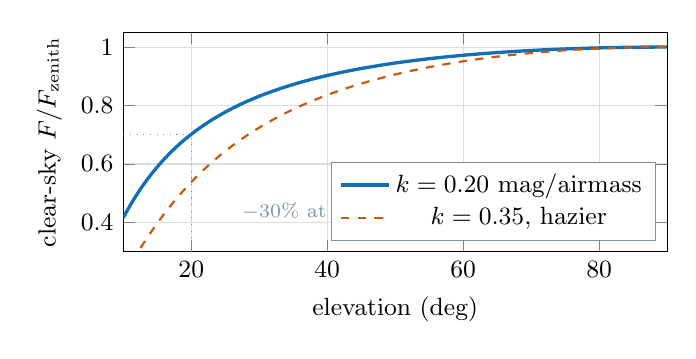
\begin{tikzpicture}
\begin{axis}[width=0.70\textwidth,height=0.36\textwidth,
  xlabel={elevation (deg)}, ylabel={clear-sky $F/F_{\text{zenith}}$},
  domain=10:90, samples=120, xmin=10,xmax=90, ymin=0.3,ymax=1.05,
  grid=both, grid style={soft!30}, tick label style={font=\small},
  label style={font=\small}, legend style={font=\small,draw=soft,at={(0.98,0.05)},anchor=south east}]
 \addplot[very thick,cam,smooth] {pow(10,-0.4*0.2/sin(x))/pow(10,-0.4*0.2)};
 \addlegendentry{$k=0.20$ mag/airmass}
 \addplot[dashed,todo,thick,smooth] {pow(10,-0.4*0.35/sin(x))/pow(10,-0.4*0.35)};
 \addlegendentry{$k=0.35$, hazier}
 \draw[soft,dotted] (axis cs:20,0.3) -- (axis cs:20,0.702);
 \draw[soft,dotted] (axis cs:10,0.702) -- (axis cs:20,0.702);
 \node[font=\scriptsize,soft,anchor=west] at (axis cs:26,0.44) {$-30\%$ at \SI{20}{\degree} with no cloud};
\end{axis}
\end{tikzpicture}
\caption{Clear-sky flux relative to the zenith, from air mass alone. A
reference built from a star's whole night mixes these elevations.}
\label{fig:airmass}
\end{figure}

\begin{table}[h]
\centering
\small
\begin{tabular}{rrrr}
\toprule
elevation & air mass $X$ & $F/F_{\text{zenith}}$ & apparent $\tau$ if compared to zenith \\
\midrule
\SI{70}{\degree} & 1.06 & 0.988 & 0.012 \\
\SI{50}{\degree} & 1.31 & 0.945 & 0.056 \\
\SI{30}{\degree} & 2.00 & 0.832 & 0.184 \\
\SI{20}{\degree} & 2.92 & 0.702 & \textbf{0.354} \\
\SI{15}{\degree} & 3.86 & 0.590 & 0.528 \\
\SI{10}{\degree} & 5.76 & 0.416 & 0.877 \\
\bottomrule
\end{tabular}
\caption{Spurious optical depth from air mass alone, $k=\SI{0.20}{mag}$ per air
mass. These are not cloud.}
\label{tab:airmass}
\end{table}

\paragraph{The effect is now measured, not predicted.} With four days of series
the extinction can be read off the data. Taking every star series with at least
forty confident samples spanning more than \SI{25}{\degree} of elevation, 188 of
them, and regressing $\ln F$ on air mass gives a median $k$ of
\SI{0.38}{mag} per air mass, with the central 68\,\% running from
\num{0.02} to \num{1.28}. Clear-sky $V$-band is about \SI{0.20}{mag}, and
\SI{70}{\percent} of the series sit above it.

Two things follow. The air-mass term is real and of the size
Table~\ref{tab:airmass} predicts, so it cannot be left in the estimator. And the
spread is the cloud signal: a whole-series regression cannot separate extinction
from weather, because cloud dims a star at whatever air mass it happens to be
at, so the fitted $k$ absorbs both and the median of \num{0.38} is an upper
bound on the true clear-sky value. That is precisely the confound the remedies
below exist to break, and it is the reason the third one is the right answer
rather than the most thorough-sounding one.

\paragraph{Three ways to fix it, in increasing quality.} The third is now
built; Sec.~\ref{sec:reference} reports what it took.
\begin{enumerate}
  \item \textbf{Bin the reference by elevation.} Compute $p_{90}$ within
    elevation bands, say \SI{10}{\degree} wide, and compare a sample only with
    its own band. Cheap, needs no model, but needs enough clear samples per band
    and still leaves a residual trend inside each band.
  \item \textbf{Fit a clear-sky curve per star.} Regress
    $\ln F$ on air mass over the upper envelope of the series, giving
    $\ln F_{\mathrm{clear}}(X) = \ln F_0 - 0.4\ln(10)\,kX$ with $F_0$ and $k$
    per star. Then $\tau$ is the departure from that curve. This is the standard
    photometric approach, is well conditioned when a star spans a range of air
    mass, and yields $k$ as a by-product, itself a useful haze diagnostic.
  \item \textbf{Fit one extinction coefficient per camera per night}, shared
    across all its stars, with per-star zero points. More constrained, more
    robust in patchy conditions, and it separates a camera-wide haze change from
    localised cloud. This is what I would recommend building.
\end{enumerate}
Until one of these is in place the stored fluxes remain correct measurements,
but the derived optical depths should not be treated as calibrated.

\section{Other open issues}

\begin{itemize}
  \item \textbf{A persistently clouded star has a depressed $p_{90}$}, so its
    own reference understates the extinction and it will look clearer than it
    is. Needs either a minimum clear-fraction test or a reference carried over
    a longer baseline than the analysis window.
  \item \textbf{Saturation is detected but not yet excluded.} A star whose
    fitted background plus amplitude reaches the top of the range has a clipped
    peak, and its flux is an underestimate; the frame view marks those with a
    cross. It is commoner than expected, and aurora is the cause: at Kiruna on
    the night of 14 September, as a display faded, 54 of 140 identified stars
    were saturated at 00:47 with the background at 172, 28 at 01:23, and one at
    01:59 with the background at 151. A bright aurora lifts the sky until the
    stars have no headroom left. These measurements must be kept out of the
    optical depth, where they would read as a fading rather than as a full
    detector.
  \item \textbf{Moonlight is measured but not corrected for.} The gradient it
    puts across a patch is now part of the fit, and its brightness is recorded
    per frame, but nothing yet uses that record. A bright Moon raises the sky
    and therefore the photon noise, so $\sigma_r$ grows and marginal stars stop
    being detectable --- which is correct behaviour --- but the clear-sky
    reference itself is still built without regard to how much moonlight each
    sample had. The stored \texttt{moon\_sky\_brightness} is a geometric proxy,
    not a scattering model; if moonlight turns out to bias the reference, it is
    the covariate to regress against first.
  \item \textbf{Detectability is computed but not yet enforced.}
    \texttt{detectable()} exists and is tested; \texttt{optical\_depth} does not
    consult it. The gate belongs at the point where a flux becomes a $\tau$, and
    until it is there an overcast frame can still read as thin cloud.
  \item \textbf{Rectilinear cameras} see under a third of the sky, so they will
    have far fewer stars and correspondingly sparse Voronoi cells.
  \item \textbf{Cell geometry.} The Voronoi tessellation is specified over star
    positions, which are image positions; cloud is at altitude. Whether cells are
    built in the image plane or on a projected shell changes the map, and should
    be decided explicitly.
  \item \textbf{Aurora contaminates the background}, not the star, but a bright
    arc through a patch will raise the fitted background and can absorb part of
    the stellar flux. Worth checking the correlation between fitted background
    and known auroral activity before trusting marginal detections.
\end{itemize}

\section{The clear-sky reference, as built}
\label{sec:reference}

\texttt{backend/extinction.rs} fits the third remedy: one coefficient per
camera, night and colour channel, with a zero point per star. The fit is a
quantile regression at the ninetieth percentile rather than least squares,
because cloud only ever subtracts and the clear sky is therefore the upper
envelope of the samples, not their middle. The choice pays for itself
numerically: for a fixed $k$ the zero point that minimises the pinball loss is
exactly the quantile of $\ln F + \beta k X$ for that star, so every zero point
profiles out analytically and what remains is a one-dimensional convex scan.
Air mass is Kasten--Young rather than $1/\sin h$, which matters because the
samples that carry the information are the low ones. A night runs from local
solar noon to noon, so one period of darkness is one fit.

\paragraph{Only a star that moves can measure the atmosphere.} This is the
lesson the archive taught, and it is worth stating plainly because it is easy
to get backwards. Every star carries its own free zero point, so a difference
between two stars at different elevations is absorbed entirely by those zero
points and says nothing about extinction. Only the air mass a star sweeps
\emph{itself} identifies $k$. On this archive most stars barely move: Kiruna
on one night showed 148 stars spanning air mass 1.1 to 4.6 across the field,
which looks like ample leverage, while individually they covered 1.08 to 1.3
and Polaris did not move at all. Fitted in that state the coefficient is
unidentified, and it showed: 42 of 100 nights returned a \emph{negative}
extinction, which is not a physical quantity. Stars that do not sweep at least
\num{0.3} in air mass are now dropped, and a night without three that do is
refused outright. A fit is refused as well when it lands on the edge of the
scan, when the coefficient comes out negative, or when the objective fails to
rise on both sides of the minimum --- the last being a direct test of whether
the night pins $k$ at all.

\paragraph{What it gives.} Run once over the whole archive, offline, the guards
accepted 151 fits and refused 745; running continuously in production a day
later, 59 fits over 20 cameras against 432 attempts (Sec.~\ref{sec:stall}). The
ratio is the honest one either way: most camera-nights genuinely do not
constrain extinction. The accepted ones land where they should. The table below
is the offline run, which covers more nights; the production figures agree with
it to within a hundredth.

\begin{center}\small
\begin{tabular}{lrrr}
\toprule
channel & fits & mean $k$ & moving stars \\
\midrule
panchromatic & 38 & 0.179 & 34.2 \\
red & 37 & 0.194 & 33.7 \\
green & 38 & 0.185 & 34.0 \\
blue & 38 & 0.191 & 32.2 \\
\bottomrule
\end{tabular}
\end{center}

\noindent The literature clear-sky value in $V$ is near \SI{0.20}{mag} per air
mass. The estimator was never told that number, and the earlier whole-series
regression on the same data gave \num{0.38}; recovering \num{0.18} is the
evidence that the envelope fit separates atmosphere from weather. Optical
depths computed from the stored references behave as they should too: on the
best-sampled night they run from \num{0.000} at the tenth percentile through
\num{0.147} at the median to \num{1.06} at the ninety-ninth, with
\SI{39}{\percent} of samples below \num{0.1}. The floor at zero is by
construction, since the reference is the ninetieth percentile of the star's own
corrected series.

\section{The reference was stalled, and why that went unnoticed}
\label{sec:stall}

A day after the reference went live its fit count had not moved: twelve fits,
the newest more than a day old, after a full period of darkness. Three separate
faults, all in \texttt{backend/starpass.rs}.

\begin{enumerate}
  \item \textbf{The pending-frame query took two minutes sixteen} on the live
    archive and ran every cycle, which is what burned a core continuously. It
    wrapped the indexed column in \texttt{julianday()}, so the index on
    observation time could not be used, and it resolved which calibration covers
    each frame through a correlated subquery over every image in the window. The
    cutoff is now compared as a string, exact because every observation time in
    the archive is RFC 3339 with a \texttt{+00:00} offset, and the calibration is
    resolved only for the few frames actually selected. Cycles now finish in
    about a second.
  \item \textbf{The cycle returned before the fit} whenever no frame was
    pending. The writer usually keeps up, so the fit was being skipped precisely
    when it was most able to run.
  \item \textbf{A refused fit recorded nothing}, so every cycle re-decided the
    same hopeless camera-nights and spent its whole budget on the first few
    cameras of a fixed order. Nothing past the tenth camera had ever been
    reached; the five cameras that held fits all sat between positions four and
    ten of that walk. Attempts are now recorded whatever their outcome, and
    cameras are visited least-recently-tried first.
\end{enumerate}

\paragraph{The methodological point.} A refusal is a result. Treating it as a
non-event, something to be re-derived on the next pass, is what let a handful of
camera-nights monopolise a bounded budget indefinitely. The same applies to the
science: a night that cannot constrain extinction has told us something about
that night, and the record of the attempt is worth as much as the record of a
success.

\paragraph{What it looks like now.} Within an hour of the fix the pass had
reached 75 cameras and stored 59 fits over 20 of them, against 432 attempts of
which 373 were refused. That ratio is the expected shape, not a fault: most
camera-nights genuinely cannot constrain extinction, for the reason in
Sec.~\ref{sec:reference}. The coefficients remain where they should be, at
\num{0.181} in the panchromatic channel and \num{0.147} to \num{0.164} in green,
red and blue, against a literature clear sky near \num{0.20}.

\paragraph{And the reason it went unnoticed for a day.} The only evidence about
the fit lived in two tables, and reading the live database from any account but
the server's own leaves its write-ahead log owned by the wrong user and takes
the whole API down; it did so twice. \texttt{GET /api/extinction} now reports
the fits, the attempts, the refusals and the coefficient by channel, so the
state of the reference can be read without touching the database. A quantity
that cannot be observed without risk will not be observed, and will therefore be
assumed.

\section{From a reference to a depth}
\label{sec:depth}

Every measurement a fitted camera-night explains now carries a vertical optical
depth, from that night's coefficient and the star's own zero point:
\[
  \tau_{\mathrm v} = \cos z\,\bigl[\ln F_{\mathrm{clear}}(X) - \ln F\bigr],
  \qquad \ln F_{\mathrm{clear}}(X) = \ln F_0 - \beta k X .
\]
The reference is the clear-sky flux \emph{at that sample's own air mass}, which
is the whole point of fitting $k$: before it, a star compared against a single
number for the night was compared against the wrong elevation.

\paragraph{A missing star is the strongest signal there is.} A star brighter
than $V=\num{3.5}$ and more than \SI{20}{\degree} above the horizon is one the
camera sees whenever the sky is clear. Its absence is therefore a measurement,
and the most informative one available: a total fading leaves exactly no flux
behind, so treating these as ``no data'' discards precisely the deepest cloud
and biases the archive towards clear. Noise-level and zero-level intensity above
background now count as a fading for such a star.

What is credited is a lower bound wherever the frame provides one. The star fell
at least as far as the faintest star that frame did detect, so
\[
  \tau_{\mathrm v} \;\ge\; \cos z\,\ln\frac{F_{\mathrm{clear}}(X)}{F_{\mathrm{faintest}}} .
\]
Where a frame detected nothing at all there is no floor to measure against and
the fading is credited as total, an optical depth of 6, under a quarter of a
percent transmitted.

\paragraph{Unless the detector is full.} Above \num{240} counts the sky itself
fills the range and a missing star is explained by the detector rather than by
the weather, so nothing is claimed. The test uses the brightest background the
frame shows rather than a typical one, which errs towards not claiming a fading:
the cost of a missed cloud is a slightly optimistic mosaic, while the cost of an
invented one is a camera wrongly suppressed.

\paragraph{And capped where the sky is already opaque.} A depth of 6 transmits
under a quarter of a percent, which is the point past which one blanket of
cloud is indistinguishable from a thicker one. Left uncapped the stored values
reached \num{40.25}, i.e.\ a transmission of $10^{-18}$, and no such number is
a measurement of weather: it is a star the reference expected at a brightness
the frame never showed, for a reason outside the model --- an obstruction, a
lens fault, a zero point fitted on a night unlike this one. Capping at the same
6 used for a total fading puts those cases where they belong, alongside ``fully
extinguished'', and stops a single unbounded value dominating any average taken
over the archive.

\paragraph{Where no number is claimed.} Three kinds of measurement are still
left null, because in each case a number would be a fiction. A faint or low star
that was not found may simply have been beyond this camera on this night. A star
whose peak is clipped reports an underestimate, so its depth would read as a
fading rather than as a full detector. And a star indistinguishable from its own
noise is not a measurement --- unless it is one of the certain ones above, where
the absence itself is the measurement.

Camera-nights the fit refuses, which are the majority, keep no depth at all.
That is the stated fallback, and it must stay one downstream: a missing depth
has to become \emph{no weight}, never a guessed one. A refit clears its window
before writing, so a depth that the new fit would refuse cannot survive as a
stale number.

\paragraph{Verified against planted cloud.} On a synthetic night whose cloud
arrives in episodes independent of elevation, the coefficient comes back at
\num{0.200} against a planted \num{0.200}, clear samples read a depth of
\num{0.0}, and clouded ones average \num{0.80} against planted cloud of
\num{0.3} to \num{1.2}. Of 180 measurements 178 carry a depth; the two
exceptions are exactly the saturated sample and the one buried in noise. On a
second night with three frames fully overcast, all nine bright, high misses are
credited at the total depth and all nine faint or low misses are left alone.

An earlier version of that test planted cloud that thickened as elevation fell.
That is the degenerate case of Sec.~\ref{sec:airmass}: no clear sky survives at
high air mass, so the fit charged the weather to the atmosphere and returned
$k=\num{0.808}$. The data was wrong, not the estimator, but it is worth
recording that this failure looks exactly like success --- depths are produced,
they are larger where the cloud was --- until the coefficient itself is checked
against something. It is the cheapest available audit of the whole chain.

\section{The instrument that reads the archive has to be checked too}
\label{sec:audit}

The fourth revision's lesson was that evidence living only in a database nobody
can safely open is not evidence, and the remedy was \texttt{/api/extinction}.
That was right as far as it went. What this revision adds is that an endpoint is
itself an instrument, and an instrument reports what it reports whether or not
it is correct.

The series endpoint's query selects twenty-seven columns, of which
\texttt{p.optical\_depth} is the twenty-second. The handler read that field
from the twenty-seventh, which is \texttt{s.sun\_elevation\_deg}. So every
optical depth it served was the elevation of the Sun at that moment --- and a
September evening at Kiruna runs from \SI{-15}{\degree} to \SI{-18}{\degree}
over a couple of hours, smoothly and monotonically. As an optical depth it is
nonsense, since it is negative; as a curve on a plot of something labelled
depth against time, it is impeccably well behaved. Five lunar and solar fields
were shifted by one in the same way, and what finally gave the whole thing away
was an illuminated fraction of $\num{-24.9}$, which cannot be a fraction of
anything. Three things from this are worth keeping.

\paragraph{A correct aggregate tells you nothing about a single value.} The
summary endpoint computes \texttt{count}, \texttt{avg} and \texttt{max} over
the column itself, so its report --- a mean depth near \num{0.45}, a maximum
sitting exactly on the cap --- was accurate the entire time. It is perfectly
possible to have a sound summary of a quantity and no ability whatsoever to
read one instance of it, and the summary will not warn you. Verification that
stops at the aggregate is not verification.

\paragraph{Positional column access has now failed twice} in this code: once
returning an empty camera registry with HTTP 200, because a fourteen-column
query was read at index fourteen, and once here. The remedy is not a better
index but a different kind of access. The query now addresses every column by
name and lives in \texttt{star\_series\_samples}, a function a test can call,
so a column inserted in the middle of the list cannot slide the rest.

\paragraph{The only test that catches this plants a different value in every
column.} Nothing weaker works. A test asserting that the flux is a flux passes
happily while the depth is a solar elevation, because both are plausible
numbers in plausible ranges, and a fixture that leaves most columns at zero or
null hides the shift entirely. The regression test seeds all twenty-seven
columns with distinct sentinels, and was confirmed to fail on precisely the
original substitution before it was accepted.

\paragraph{What the corrected endpoint shows.} Depths now read one at a time,
and they behave. At Klin, the star $11.03066{+}56.38234$ carries a median
$\tau$ of \num{0.51} in blue, \num{0.49} in green, \num{0.43} in red and
\num{0.47} in the mean channel; at Gulkevichi, $0.61619{+}53.89693$ gives
\num{0.14}, \num{0.16}, \num{0.03} and \num{0.16}. Cloud extinction is close
to achromatic, so four independently fitted references --- separate quantile
fits, separate coefficients, separate zero points --- agreeing to within
\num{0.05} is evidence about the reference itself, and not merely evidence that
it is self-consistent. It is the cheapest audit available of everything upstream
of the number.

\section{Where the cloud weight now has to go}
\label{sec:weightpath}

The composite was rebuilt on 11 September to compose camera layers in the
browser, and that changes the answer this memo gave for applying the weight.
There are now two places a factor can live, and they are not
interchangeable.

\begin{enumerate}
  \item \textbf{Baked into the published mesh, per vertex}
    (\texttt{backend/publish\_layers.rs}). This carries the factors that vary
    across an image: the magnetic-axis weight, the zenith taper and the
    mask-edge fade. One float per vertex, computed once when the layer is
    published.
  \item \textbf{Applied per layer in the browser}
    (\texttt{src/composition-rules.ts}, \texttt{cameraWeightScale}). This
    carries the factors that are one number for a whole image: the solar taper
    and the operator's quality weight $2^{n}$. The browser recomputes the solar
    elevation from the camera's position and the frame's epoch with the same
    equations as \texttt{backend/geometry.rs}.
\end{enumerate}

A cloud weight is one number per camera per frame, so by shape it belongs in
the second group. But it differs from both of its neighbours there in a way
that matters: the solar taper and the quality weight can be \emph{computed} in
the browser from data it already has, and an optical depth cannot. It is a
measurement. It therefore has to be published --- carried per frame in the
layer manifest, beside the texture and geometry URLs --- and multiplied into
\texttt{cameraWeightScale} as a third factor. The server-side composite in
\texttt{publish.rs} still exists and still applies the full chain, so the same
factor has to enter there too, or the admin and public views will disagree
about which camera won a pixel. Keeping those two in step is the whole reason
\texttt{composition-rules.ts} was split out as a shared module, and the cloud
term should follow that pattern rather than work around it.

\section{A first cloud weight in the composite, and why it is provisional}
\label{sec:cloudweight}

A weight built from the star fading now multiplies both composites. It is the
first thing in this memo that changes a picture rather than a table, and it is
deliberately the simplest quantity that could: not the stored optical depth of
Sec.~\ref{sec:depth}, but the fading factor the frame view already draws ---
each star's present flux against the best that camera has ever recorded for it.
That keeps the first version legible and leaves the depth, with its refusals and
its gates, for when this one has been looked at.

\paragraph{The field.} Each usable star owns the region of the image closer to
it than to any other, and carries its own fading flat across that cell. Across a
boundary the two cells are blended over \SI{10}{px} with the same smooth step
$f_s$ used everywhere else in the weight chain, and only where the cell is
larger than that band --- inside \SI{10}{px} of its own star a cell keeps its
own value, since a transition wider than the cell would erase the measurement
it exists to carry. The result is continuous, equals a star's own fading over
almost all of its cell, and equals the mean of two neighbours on the boundary
between them.

A Hann taper across each cell, from full trust at the star to none at its
boundary, is implemented and \emph{off}. The question it answers is real --- a
star two hundred pixels away is weaker evidence than one overhead --- but it has
not been looked at on real frames and it interacts with the boundary blend in a
way nobody has examined. Leaving it off makes the field say exactly what was
measured, and confines the smoothing to where it was asked for.
\texttt{GAIA\_CLOUD\_HANN=1} restores it without a rebuild, and both manifests
publish which of the two built the mosaic, so a picture always says what it was
made with.

\paragraph{Three stars, at least.} The first live publish showed why a floor on
the number of stars is not a detail: ten fields in sixteen were a single value
across the whole image, and six of those dimmed an entire all-sky camera on one
star's fading, one of them to seven percent. A lone star is very nearly absence
of measurement, and the field carries no spatial information at all below three
points. Frames with fewer now publish no field, and their layers composite
exactly as they did before --- the same floor, and for the same reason, as the
clear-sky fit uses.

Two further consequences are worth stating because they are choices, not accidents. The
weight is floored at \num{0.02} rather than reaching zero: with a single
contributing camera the per-pixel normalization divides the weight out again, so
a floor confines the effect to overlaps, which is the only place a preference
between cameras means anything. And a frame with no usable stars gets no field
at all rather than a field of zeros --- it composites exactly as it did before,
because absence of measurement is not measurement of cloud.

\paragraph{The denominator.} The factor multiplies the weight and never the
pixel value, so it enters the normalizing sum with everything else. Server-side
the same variable multiplies the colour and accumulates in the fourth channel;
in the browser the fragment shader forms the product once and uses it for both
the colour sum and the weight sum. There is no path by which the two can
disagree.

\paragraph{Why it is preliminary.} A star disappears from the photometry for
two reasons that are identical in the data and opposite in meaning:

\begin{itemize}
  \item bright aurora lifts the background until the star's peak is clipped ---
    and the sky above is \emph{clear};
  \item thin cloud lit by the Moon lifts the background until the star's peak is
    clipped --- and the sky above is \emph{not}.
\end{itemize}

Both give a similar peak intensity and a similar background. No rule written
today separates them, so saturated fits are excluded from the field rather than
counted either way. That is conservative in one direction only: it biases the
archive towards believing the sky is clear, which is exactly the bias a cloud
weight exists to remove. Before this can be settled the archive has to collect
measured responses under both conditions --- aurora over a clear sky, and
moonlit thin cloud --- and they have to be compared. Until then the weight is
useful for seeing the effect and wrong to quote. It is published with that
caveat attached in both manifests, and \texttt{GAIA\_CLOUD\_WEIGHT=0} turns it
off without a rebuild.

\section{What remains to be built}
\label{sec:remains}

\begin{enumerate}
  \item \textbf{Spend the optical depth.} A cloud weight now reaches both
    composites (Sec.~\ref{sec:cloudweight}), but from the fading factor rather
    than from the stored depth: the depth carries the clear-sky reference and
    the air-mass correction the fading does not, and it refuses to exist where
    the night could not be fitted. Moving the field onto it is the next step,
    and the two can be compared directly since they are the same shape.
  \item \textbf{Separate aurora from moonlit thin cloud}, which is what blocks
    saturated stars from contributing at all (Sec.~\ref{sec:cloudweight}).
    This wants collected responses under both conditions before any rule.
  \item \textbf{Apply the weight.} \texttt{cloud\_weight} exists and is tested:
    $w=\text{floor}+(1-\text{floor})e^{-\tau}$, strictly positive so a single
    contributing camera normalises back to full strength and no hole is punched.
    It is not yet a factor in \texttt{publish.rs}. It multiplies the weight, not
    the pixel value, unlike the intensity equalization gains. The composite
    weight is now a product of five factors --- magnetic axis, zenith taper,
    mask-edge fade, solar taper and the operator's per-camera quality setting
    $2^{n}$ --- so the cloud term is a sixth factor of the same kind, and the
    cache keys must take it the way they now take the quality weights. It has to
    be applied in both composites, which since 11 September means two places:
    see Sec.~\ref{sec:weightpath}.
  \item \textbf{Surface the noise in the panel.} $\sigma_r$ and the
    signal-to-noise ratios are stored and served by the API but not drawn; a
    brightness series without its noise band cannot be read honestly. The
    distributions now drawn beside it (total intensity, peak and background, per
    colour channel, over the whole archive for one star) are the natural place
    to put it.
  \item \textbf{Voronoi cloud-cover output.} The tessellation itself is built
    and drawn: cells are cut to the camera's own projected horizon rather than to
    the frame, since a fisheye's corners are ground and housing, and each
    boundary takes the colour of the more faded of the two stars across it, so a
    clouded star is ringed in dark red all the way round. What remains is to
    assign each cell an optical depth rather than a relative brightness, feather
    the edges with the $\psi$-based smooth step at \SI{10}{\percent} of cell
    width, and publish the map as an image in the browse-history panel.
  \item \textbf{Let the pass reach the whole archive.} It looks back
    \SI{48}{\hour} by default, which keeps it current but leaves the history
    unmeasured. A backfill wants a wider window and a night-by-night sweep.
  \item \textbf{Per-frame pointing correction} for the cameras that need it,
    with the standing per-camera offset used as a recalibration flag for the
    rest (Sec.~\ref{sec:writer}).
\end{enumerate}

\section{Where the code is}

\begin{itemize}
  \item \texttt{backend/starphot.rs} --- catalogue, ephemeris, forward
    projection, field test, Gaussian fit on a bilinear sky, residual scatter and
    detectability, lunar ephemeris and state, percentile, optical depth, cloud
    weight, storage, variation metric.
  \item \texttt{backend/schema.sql} --- the \texttt{star\_photometry} and
    \texttt{frame\_sky} tables and their indices.
  \item \texttt{backend/starpass.rs} --- the writer: frame selection, the sky
    record, cadence thinning, the lens-model cache, the background loop and the
    nightly refit of the clear-sky reference.
  \item \texttt{backend/extinction.rs} --- air mass, the observing night, the
    quantile fit, the identifiability guards, and the optical depth that
    follows from a fit.
  \item \texttt{backend/publish\_layers.rs}, \texttt{src/composition-rules.ts}
    --- the two halves of the composite weight, and where a cloud factor has to
    be added (Sec.~\ref{sec:weightpath}).
  \item \texttt{backend/main.rs} --- the star endpoints: \texttt{stars},
    \texttt{stars/series} (whose query lives in \texttt{star\_series\_samples},
    addressed by column name, Sec.~\ref{sec:audit}),
    \texttt{stars/frame} with its camera field outline
    and saturation flag, \texttt{stars/nights}, \texttt{stars/distribution} for
    the whole-archive histograms, and \texttt{/api/extinction}, which reports
    the state of the clear-sky reference without anyone having to open the
    database.
  \item \texttt{src/voronoi.ts}, \texttt{src/histogram.ts} --- the tessellation
    cut to the camera's field, and the binning behind the distributions.
  \item \texttt{deploy/gaia-revontuli.service} --- the \texttt{GAIA\_STARPHOT\_*}
    settings, all of them overridable without a rebuild.
  \item \texttt{app/page.tsx}, \texttt{app/globals.css} --- the Star photometry
    panel in the Cameras tab: brightness and background series on a shared time
    axis, and a frame scatter coloured by brightness variation.
\end{itemize}

\end{document}
